\begin{center}
	
	\begin{tabular}{rp{16cm}lp{20cm}}%{rl}
		
		% after \\: \hline or \cline{col1-col2} \cline{col3-col4} ...
		
		论文地址:& \href{https://arxiv.org/pdf/2002.07033.pdf}{https://arxiv.org/pdf/2002.07033.pdf} \\
		来源:& L@S, 2020 \\
		作者:& Youngduck Choi, et al. \\
		单位:& Riiid! AI Research, Yale University, University of Michigan, UC Berkeley \\
		源码:& \href{https://github.com/arshadshk/SAINT-pytorch}{SAINT} \\
		
		%  slides:& \href{http://yunshengb.com/wp-content/uploads/2017/03/nips_2018_r2l_workshop_talk.pdf}{{\footnotesize Convolutional Set Matching for Graph Similarity}}\\
		
		关键词:& \textbf{Knowledge Tracing, Student assessment, Transformer} \\
		
		写于:& \date{2021-09-22}
		
	\end{tabular}
	
\end{center}

该论文\cite{youngduck2020towards}针对当前Transformer和基于注意力的Knowledge Tracing模型的缺点,提出了基于Transformer的Knowledge Tracing模型 --- Separated Self-AttentIve Neural Knowledge Tracing(SAINT)。在SAINT中,练习和回答的embedding序列分别进入encoder和decoder部分。

\paragraph{问题定义}
\begin{figure}[h]
	\centering
	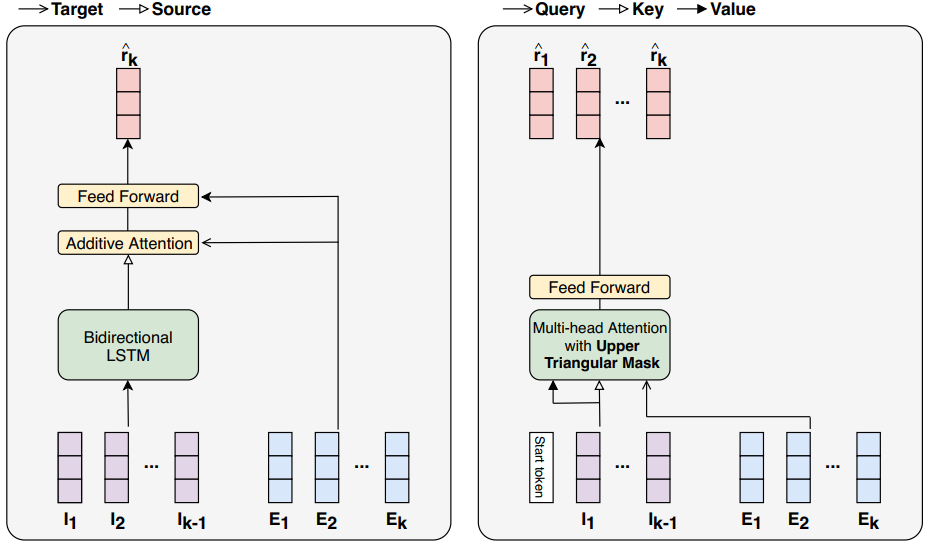
\includegraphics[width=.65\textwidth]{pics/saint-prev-methods.png}
	\caption{Architectures of Previous Methods}
	\label{fig:saint-prev}
\end{figure}
提出SAINT是为了解决现有的基于注意力的Knowledge Tracing的模型(如Fig.\ref{fig:saint-prev}所示)的两个局限:
\begin{itemize}
	\item 注意力层太浅,难以捕捉练习和回答之间复杂的关系
	\item 没有使用合适的方法构造注意力中的query, key, value
\end{itemize}

SAINT将练习和回答的embedding分别输入到SAINT的encoder和decoder部分(注意与Fig.\ref{fig:saint-prev}区别)。

形式化定义:

学生的行为序列:$\boldsymbol{I}_1, ..., \boldsymbol{I}_n$,其中$\boldsymbol{I}_i = \{E_i, R_i\}$,$E_i$表示第$i$个交互中的练习的信息,$R_i$表示学生此次练习的作答信息。SAINT的目标:$P(R_k = 1 | \boldsymbol{I}_1, ..., \boldsymbol{I}_{k-1}, E_k)$。

\paragraph{SAINT}
\begin{figure}[h]
	\centering
	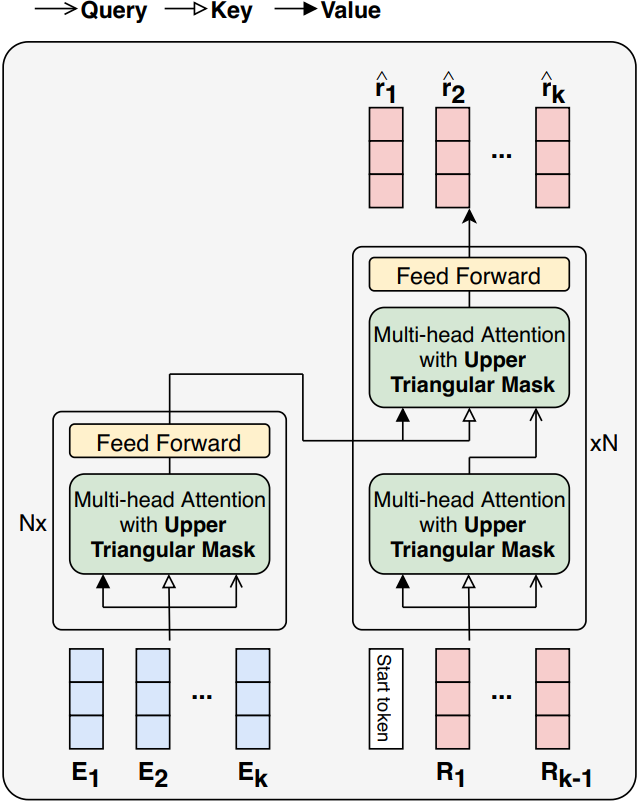
\includegraphics[width=.38\textwidth]{pics/saint.png}
	\caption{Architecture of SAINT}
	\label{fig:saint}
\end{figure}
SAINT的模型结构如Fig.\ref{fig:saint}所示。$E_i, R_i$可以包含多种属性,如ID、类别、做题化的时间等,SAINT会先将原始的信息转换为embedding,则输入到SAINT是转换后的embedding序列。

SAINT的工作流程基本与Transformer一致。

论文中使用的数据集为\href{https://github.com/riiid/ednet}{EdNet}(关于英语教育,规模较大),使用的指标是AUC。

\paragraph{总结}

\begin{itemize}
	\item 将练习和回答分别作为encoder和decoder的输入,基于Transformer预测学生的知识水平
	%\item 
	
\end{itemize}

